\documentclass[template=tabling,11pt,headonall]{azmoon}
\usepackage{xepersian}
\settextfont{Yas}
\setdigitfont{Yas}

\printanswers

\teacher{آقای باغبان}
\teachertitle{دبیر}
\city{لارستان}
\schooltitle{دبیرستان}
\school{فارابی}
\grade{هشتم}
\branch{شهید جعفری‌نژادان}
\topic{ریاضی}
\examdate{96/12/23}
\answertime{60 دقیقه}
\begin{document}
	\begin{questions}
		\nointerlineskip%
		\vskip-\baselineskip
		\section{سوالات درست یا نادرست}
		\question[1]{
			عبارت‌ درست را با ‎\truesym و عبارت نادرست را با ‎\falsesym مشخص کنید.
			\begin{truefalse}[2]
				\itemt{جمله‌های $3x^2y$ و $-5yx^2$ متشابه هستند.}
				\itemf{حاصل‌ضرب عدد فرد در عدد زوج عددی فرد است.}
				\itemt{تفاضل هر عدد دورقمی از مقلوبش مضرب 9 است.}
				\itemt{حاصل‌جمع عدد فرد با عدد زوج عددی فرد است.}
			\end{truefalse}
		}
		\section{سوالات جاخالی}
		\question[2]{%
			جاهای خالی را با عبارت مناسب پر کنید.
			\begin{parts}[2]
				\part{حاصل‌جمع سی و هفت عدد فرد عددی \fillin[1.5cm]{فرد} است.}
				\part{عبارت $-(a-b+c)$ برابر \fillin[2.5cm]{$-a+b-c$} است.}
				\part{اگر برآیند دو بردار برابر بردار صفر شود، گوییم که دو بردار \fillin[1.5cm]{قرینه} یکدیگرند.}
				\part{ضریب عددی جمله $\dfrac{-7ax}{3}$ برابر \fillin[1cm]{$\dfrac{-7}{3}$} است.}
			\end{parts}
		}
		\section{سوالات چهارگزینه‌ای}
		\question[0.5]{%
			اگر 
			$\vec{a}=\pvector{-1}{3}$
			و 
			$\vec{b}=\pvector{2}{-6}$ 
			حاصل 
			$2‎\vec{a}+\vec{b}‎$ برابر با کدام گزینه است؟
			\begin{fourchoice}
				\choice{$\pvector{3\\1}$}
				\choiceok{$\pvector{0\\0}$}
				\choice{$\pvector{1\\1}$}
				\choice{$\pvector{-1\\-1}$}
			\end{fourchoice}
		}
		\question[0.5]{%
			جمله‌ی $5xy^2$
			با کدام گزینه متشابه است؟
			\begin{fourchoice}
				\choiceok{$-2y^2x$}
				\choice{$5xy$}
				\choice{$5yx^2$}
				\choice{$5x^2y^2$}
			\end{fourchoice}
		}
		\section{سوالات بلندپاسخ}
		\question[3]{%
			حاصل عبارت‌های زیر را به‌دست آورید.
			\begin{LTR}
				\begin{parts}[2]
					\part{$2xy-5x-7xy-7x=$ \answer{$-5xy-12x$}}
					\part{$(x-4)(x+7)=$ \answer{$x^2+7x-4x-28=x^2+3x-28$}}
					\numcols{1}
					\part{$(3x+2y)(3x-2y)=$ \answer{$9x^2-6xy+6xy-4y^2=9x^2-4y^2$}}
					\part{$(2x-3y)^2=$ \answer{$(2x-3y)(2x-3y)=4x^2-6xy-6xy+9y^2=4x^2-12xy+9y^2$}}
				\end{parts}
			\end{LTR}	
		}
		\question[1.5]{%
			با توجه به جدول زیر و رابطه $y=2x+3$ جاهای خالی را پر کنید.
			\begin{LTR}
				\begin{tabular}{c|cccc}
					$x$ & $-2$ & $-\dfrac{3}{2}$ & \fillin[0cm]{$\dfrac{-1}{2}$} & \fillin[0cm]{$-3$} \\ \hline
					$y$ & \fillin[0cm]{$-1$} & \fillin[0cm]{$0$} & $2$ & $-3$
				\end{tabular}
			\end{LTR}
		}
		%	\noprintlinesep
		\question[2]{%
			عبارات زیر را تجزیه کنید.
			\begin{LTR}
				\begin{parts}[2]
					\part{$4x^2y+6xy^2=$ \answer{$2xy(2x+3y)$}}
					\part{$8x^2y^3-4xy^2=$ \answer{$4xy^2(2xy-1)$}}
					\part{$42xy^3-35x^2y^2=$ \answer{$7xy^2(6y-5x)$}}
				\end{parts}
			\end{LTR}
		}
		%\printlinesep
		\question[1.5]{%
			با تجزیه صورت و مخرج، کسر زیر را ساده کنید.
			\begin{LTR}
				$\dfrac{a^2b-ab^2}{a^3b^2-a^2b^3}=$ \answer{$\dfrac{ab\cancel{(a-b)}}{a^2b^2\cancel{(a-b)}}=\dfrac{1}{ab}$}
			\end{LTR}
		}
		\question[1.5]{%
			معادله‌های زیر را حل کنید.
			\begin{LTR}
				\begin{parts}
					\part{$\pvector{2\\7}+\vec{x}=\pvector{5\\3}$}
					\vspace{.2cm}
					\part{$2\vec{x}+\pvector{3\\1}=9\vec{i}-5\vec{j}$}
				\end{parts}
			\end{LTR}
		}
		\question[2]{%
			معادله‌های زیر را حل کنید.
			\begin{LTR}
				\begin{parts}[4]
					\part{
						$2x+3=-5$
						\answer[2.5cm]{$\\2x=-3-5\\2x=-8\\x=\dfrac{-8}{2}\\x=-4$}
					}
					\part{$\dfrac{2}{3}x-\dfrac{1}{2}=\dfrac{1}{6}$}
					\part{$\dfrac{x+1}{2}=\dfrac{x+1}{3}$}
					\part{$\dfrac{1}{2}-\dfrac{2x-1}{4}=\dfrac{3}{4}$}
				\end{parts}
			\end{LTR}
		}
		\question[1]{%
			در تساوی‌های زیر $x$ و $y$ را به‌دست آورید.
			\begin{LTR}
				\begin{parts}[2]
					\part{$\pvector{5\\6}+\pvector{x\\y}=\pvector{2\\8}$}
					\part{$\pvector{3\\y}+\pvector{x\\-5}=\pvector{4\\7}$}
				\end{parts}
			\end{LTR}
		}
		\question[2.5]{%
			با توجه به بردارهای $‎\vec{a}‎$، $‎\vec{b}‎$ و $‎\vec{c}‎$ که در شکل زیر مشخص شده است، بردار $\vec{v}=2\vec{a}+\vec{b}-\vec{c}$ را به روش هندسی و جبری به‌دست آورید. کدام روش برای رایانه‌ای شدن مناسب‌تر است؟ چرا؟‎
			\definecolor{cqcqcq}{rgb}{0.7529411764705882,0.7529411764705882,0.7529411764705882}
			\begin{LTR}
				\hspace{.5cm}
				\begin{tikzpicture}[line cap=round,line join=round, x=.5cm,y=.5cm]
				\draw [color=cqcqcq,, xstep=.5cm,ystep=.5cm] (0,0) grid (9,7);
				\clip(0.,0.) rectangle (9.,7.);
				\draw [->,line width=1.pt] (4.,5.) -- (6.,6.);
				\draw [->,line width=1.pt] (7.,7.) -- (8.,5.);
				\draw [->,line width=1.pt] (2,5) -- (5,7);
				\answer{%
					\draw [->,line width=1.pt, color=blue] (0,2) -- (4,4);
					\draw [->,line width=1.pt, color=blue] (4,4) -- (5,2);
					\draw [->,line width=1.pt, color=blue] (5,2) -- (2,0);
					\draw [->,line width=1.pt, color=green] (0,2) -- (2,0);
				}
				%		\begin{scriptsize}
				\draw[color=black] (5,5.95) node {$\vec{a}$};
				\draw[color=black] (7.75,6.3) node {$\vec{b}$};
				\draw[color=black] (3.6,6.5) node {$\vec{c}$};
				%		\end{scriptsize}
				\end{tikzpicture}
			\end{LTR}
		}
		\question[1]{%
			بردارهای داده  شده را روی امتدادهای رسم شده تجزیه کنید.
			\begin{LTR}
				\hspace{1cm}
				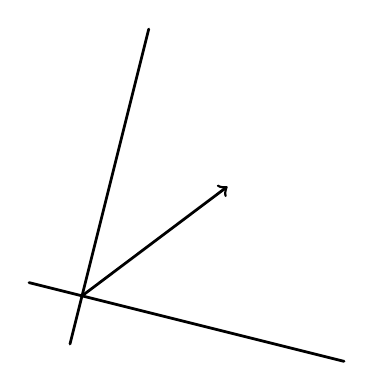
\begin{tikzpicture}[line cap=round,line join=round,x=1.0cm,y=1.0cm]
				\draw [line width=1.pt] (1.,1.)-- (2.,5.);
				\draw [line width=1.pt] (0.48,1.78)-- (4.48,0.78);
				\draw [->,line width=1.pt] (1.1529411764705884,1.6117647058823532) -- (3.,3.);
				\end{tikzpicture}
				\hfill
				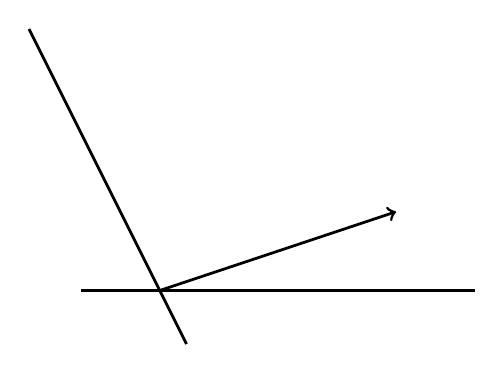
\begin{tikzpicture}
				\draw [line width=1.pt] (7.34,4.32)-- (9.34,0.32);
				\draw [line width=1.pt] (8.,1.)-- (13.,1.);
				\draw [->,line width=1.pt] (9.,1.) -- (12.,2.);
				\end{tikzpicture}
				\hspace{1cm}
			\end{LTR}
		}
	\end{questions}
\end{document}